\documentclass[12pt, letterpaper]{article}
%\documentclass[10pt, letterpaper, twocolumn]{article}

% Images
\usepackage{graphicx}
\graphicspath{{images}}

% For positioning figures (eg. images) with [H]
\usepackage{float}

% For styling figure captions
\usepackage{subcaption}
\captionsetup{labelfont=bf, textfont=it, font=footnotesize}

% For styling headers/sections
\usepackage{titlesec}
\titlelabel{\thetitle.\quad}
\titleformat*{\section}{\large\bfseries} % Custom font/size for sections

% Header on each page, and footer
\usepackage{fancyhdr}
\pagestyle{fancy}
\fancyhf{} % sets both header and footer to nothing
\renewcommand{\headrulewidth}{0pt}
\fancyhead[CO]{\footnotesize\textit{Luis F. / Lifecycle Project:
LG 50LB5800}}
\fancyfoot[CO]{\thepage} % page numbers

% Bibliography
\usepackage{csquotes}
\usepackage[style=mla]{biblatex}
\addbibresource{main.bib}

% Links
\usepackage{hyperref}
\hypersetup{colorlinks=true, linkcolor=blue, urlcolor=cyan, citecolor=black}
\urlstyle{same}

% Custom commands
\newcommand\todo[1]{{\color{red}{\footnotesize[TODO: #1]}}} % show todo's in red
%\newcommand\todo[1]{} % to remove all todo's

\begin{document}

%\title{\vspace{-3em}\Huge{\textbf{Lifecycle Project: LG 50LB5800}}}
%\title{\vspace{-3em}\Large{\textbf{Lifecycle Project: LG 50LB5800}}}
\title{\vspace{-3em}\Large{\textbf{\mbox{\hspace{-0.25em}Lifecycle
Project: LG 50LB5800}}}} % the mbox and hspace help to fit in one line
\author{\small{Luis F.}}
\date{\vspace{-0.5em}\small{December 2024}}

\maketitle

% Nicer formatting of the abstract enclosed in lines
\renewenvironment{abstract}
{
  \begin{quote}
  \noindent \rule{\linewidth}{.5pt}\par{\bfseries \abstractname.}}
  {\\ \noindent \rule{\linewidth}{.5pt}\medskip
  \end{quote}
}

\vspace{-2em}
% \begin{abstract}\small\itshape
% blah blah blah
% \end{abstract}

% Do I even need a ToC for such a small paper?
\tableofcontents

\section{Criterion A: 3D Design Write-up}

For my Digital Societies Lifecycle Project, I decided to research the
lifecycle of an LG 50LB5800 TV. I have one of these at home, so it is
convenient to measure and model. Since I found it being thrown away,
and it currently doesn't work, I'm free to open it up and see inside
if I want to.

\begin{figure}[H]
  \medskip
  \centering
  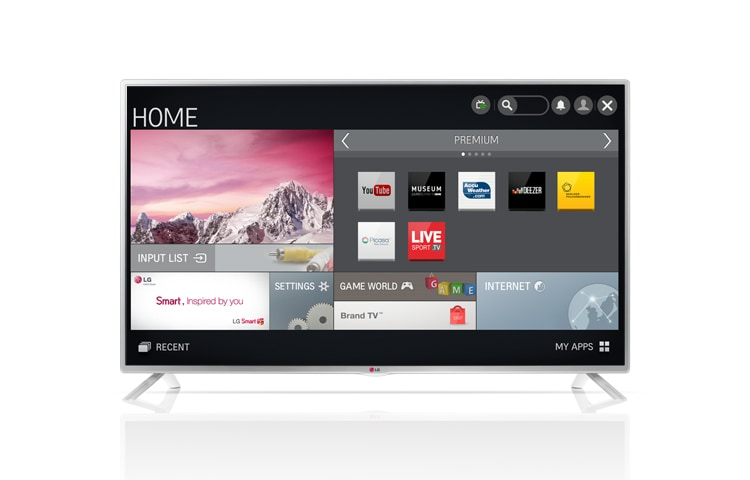
\includegraphics[width=1\linewidth]{lg-50LB5800}
  \caption{50LB5800 LG Smart TV~\autocite{unknown-author-no-dateB}.}
  \medskip
  \label{fig:lg-50LB5800}
\end{figure}

I decided to model the TV using CAD software, as I had previous
experience using
\href{https://www.autodesk.com/products/fusion-360/overview}{Fusion
360} and thought it was the most appropriate choice for this project.
However, I had issues with licensing and downloading Fusion 360, so I
decided to try out FreeCAD. \href{https://www.freecad.org}{FreeCAD}
is an open-source parametric 3D modeling
software~\autocite{jolahde-2018}. It has a variety of online
resources, like tutorials and documentation, so I was able to learn
it quickly enough for this project.

I started off the model by making a 2D sketch, and making a
rectangle. This would be the base frame of the television. I then
measured the frame of the television using a metre stick, to ensure
the design was of a one-to-one scale. After the frame was done, I
sketched the TV screen. This was more challenging as the only
measurement I had was the diagonal length of the screen being 50
inches, however I was able to make an accurate sketch using constraints.

\begin{figure}[H]
  \medskip
  \centering
  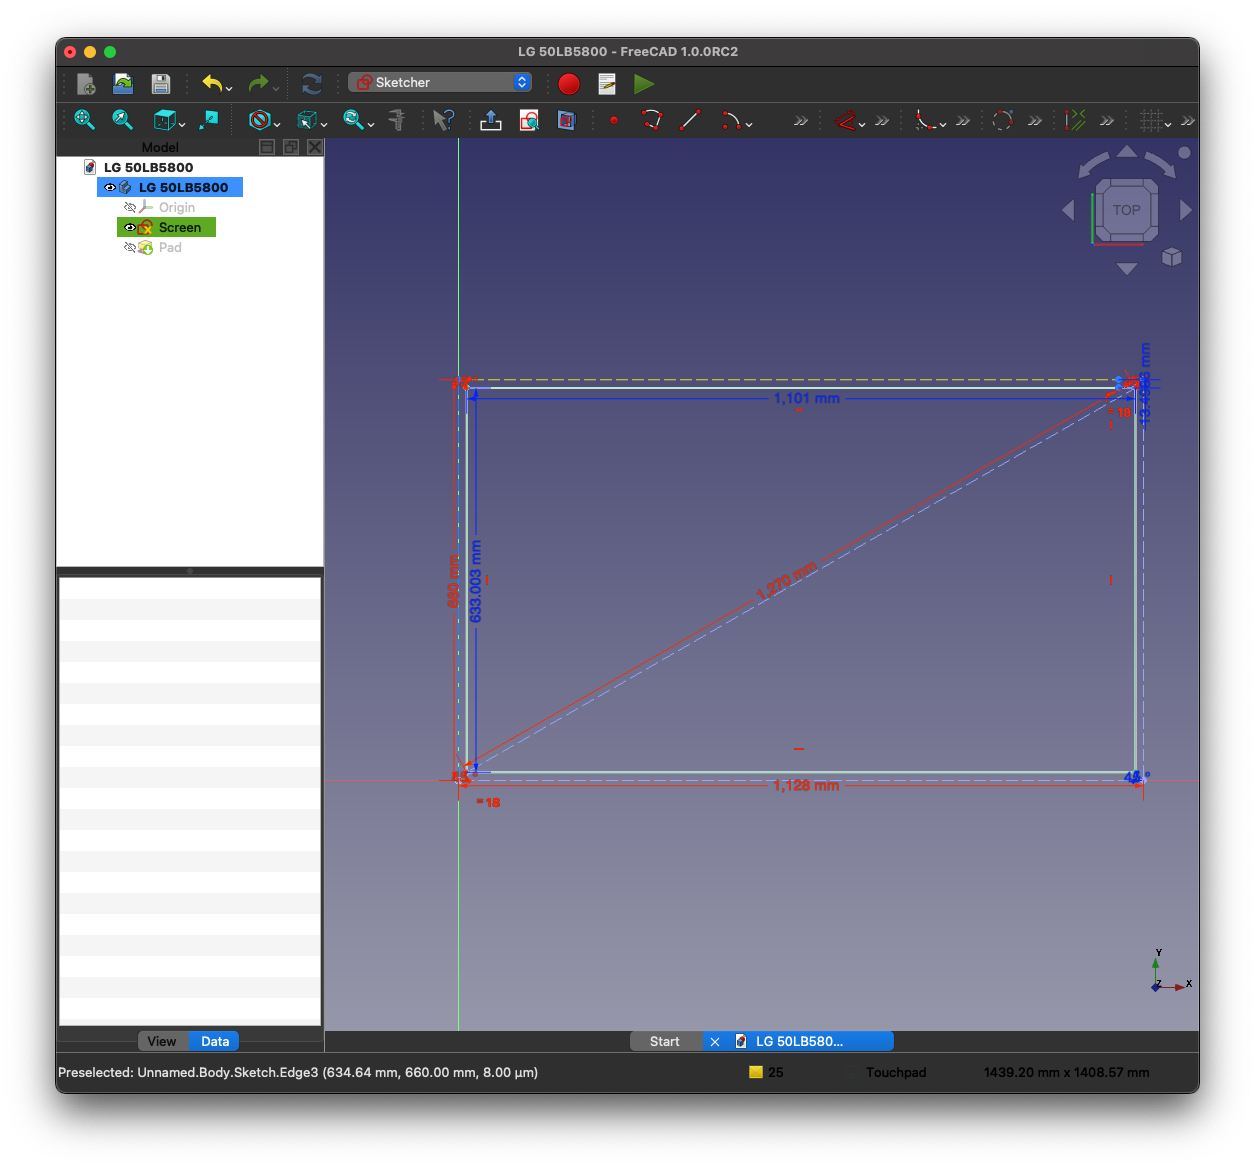
\includegraphics[width=1\linewidth]{a1}
  \caption{Sketching the TV screen in FreeCAD.}
  \medskip
  \label{fig:a1}
\end{figure}

Then I extruded, or in FreeCAD terms ``padded'', the frame. I had to
measure the thickness of the TV to make it to scale.

\begin{figure}[H]
  \medskip
  \centering
  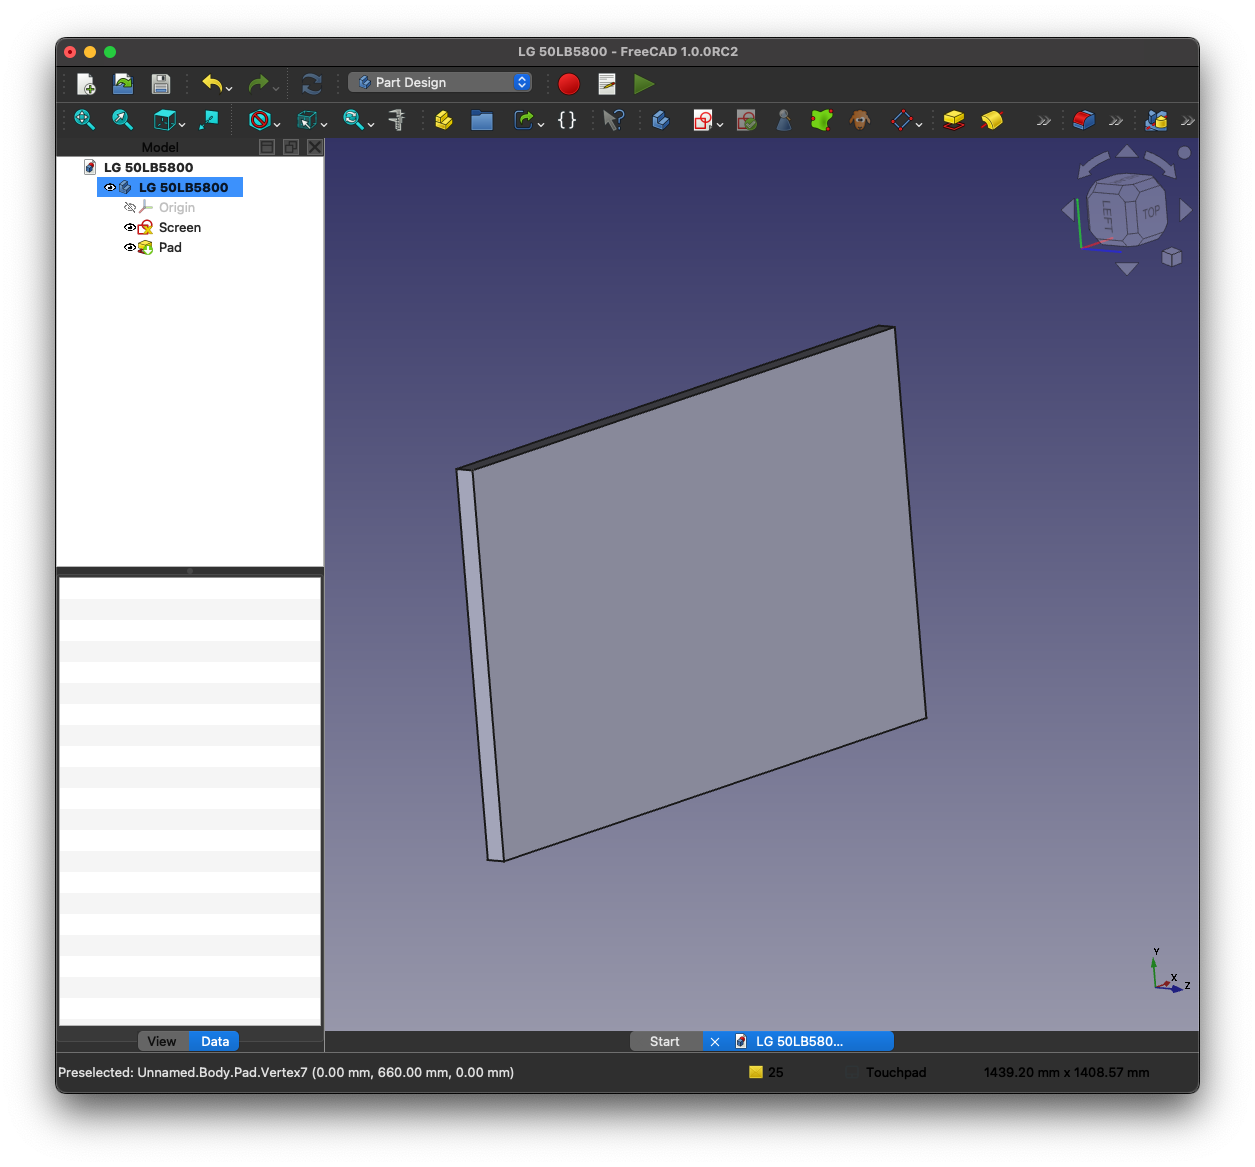
\includegraphics[width=1\linewidth]{a2}
  \caption{Modeling the base of the TV in FreeCAD.}
  \medskip
  \label{fig:a2}
\end{figure}

By taking more measurements and using these basic operations
(sketching and padding, and also a bit of filleting), I was able to
arrive at my final 3D model.

\begin{figure}[H]
  \medskip
  \centering
  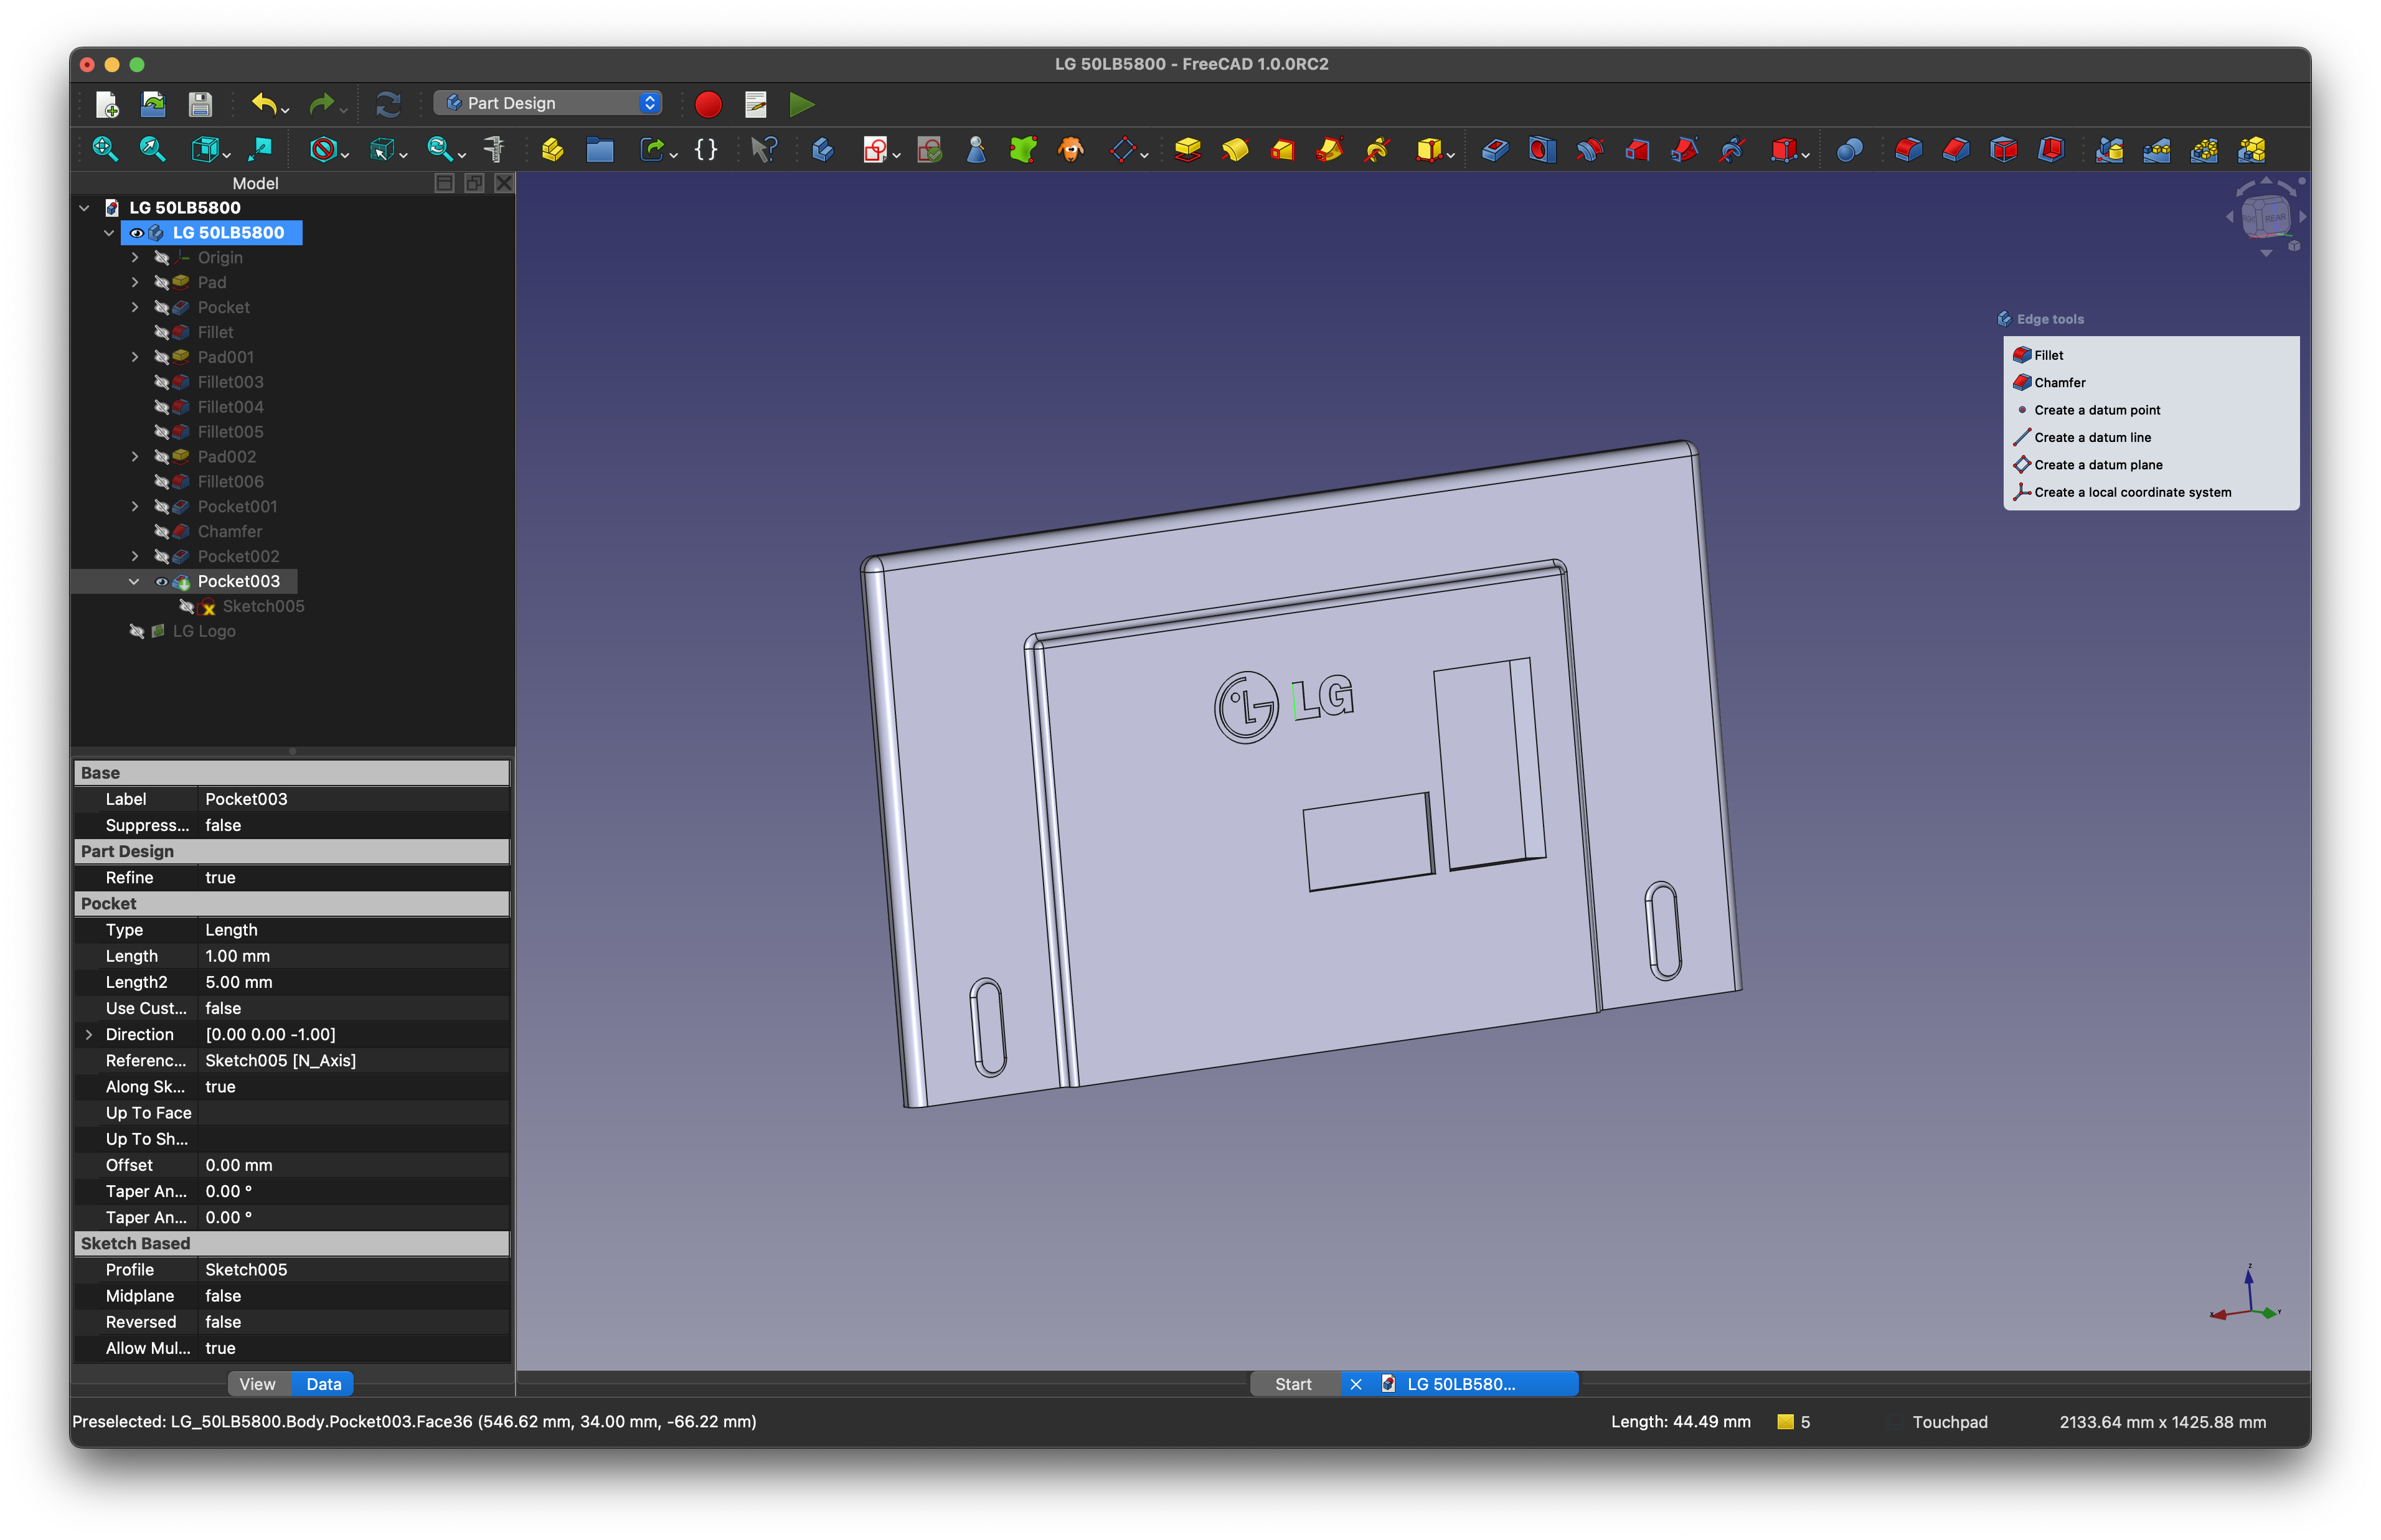
\includegraphics[width=1\linewidth]{a3}
  \caption{My final 3D model of a 50LB5800 LG Smart TV.}
  \medskip
  \label{fig:a3}
\end{figure}

I decided to add the LG logo to the back of my model, just like the
real one has. I sketched the logo on top of a reference image of the
logo using regular sketch tools and B-splines for the curves of the G.

\begin{figure}[H]
  \medskip
  \centering
  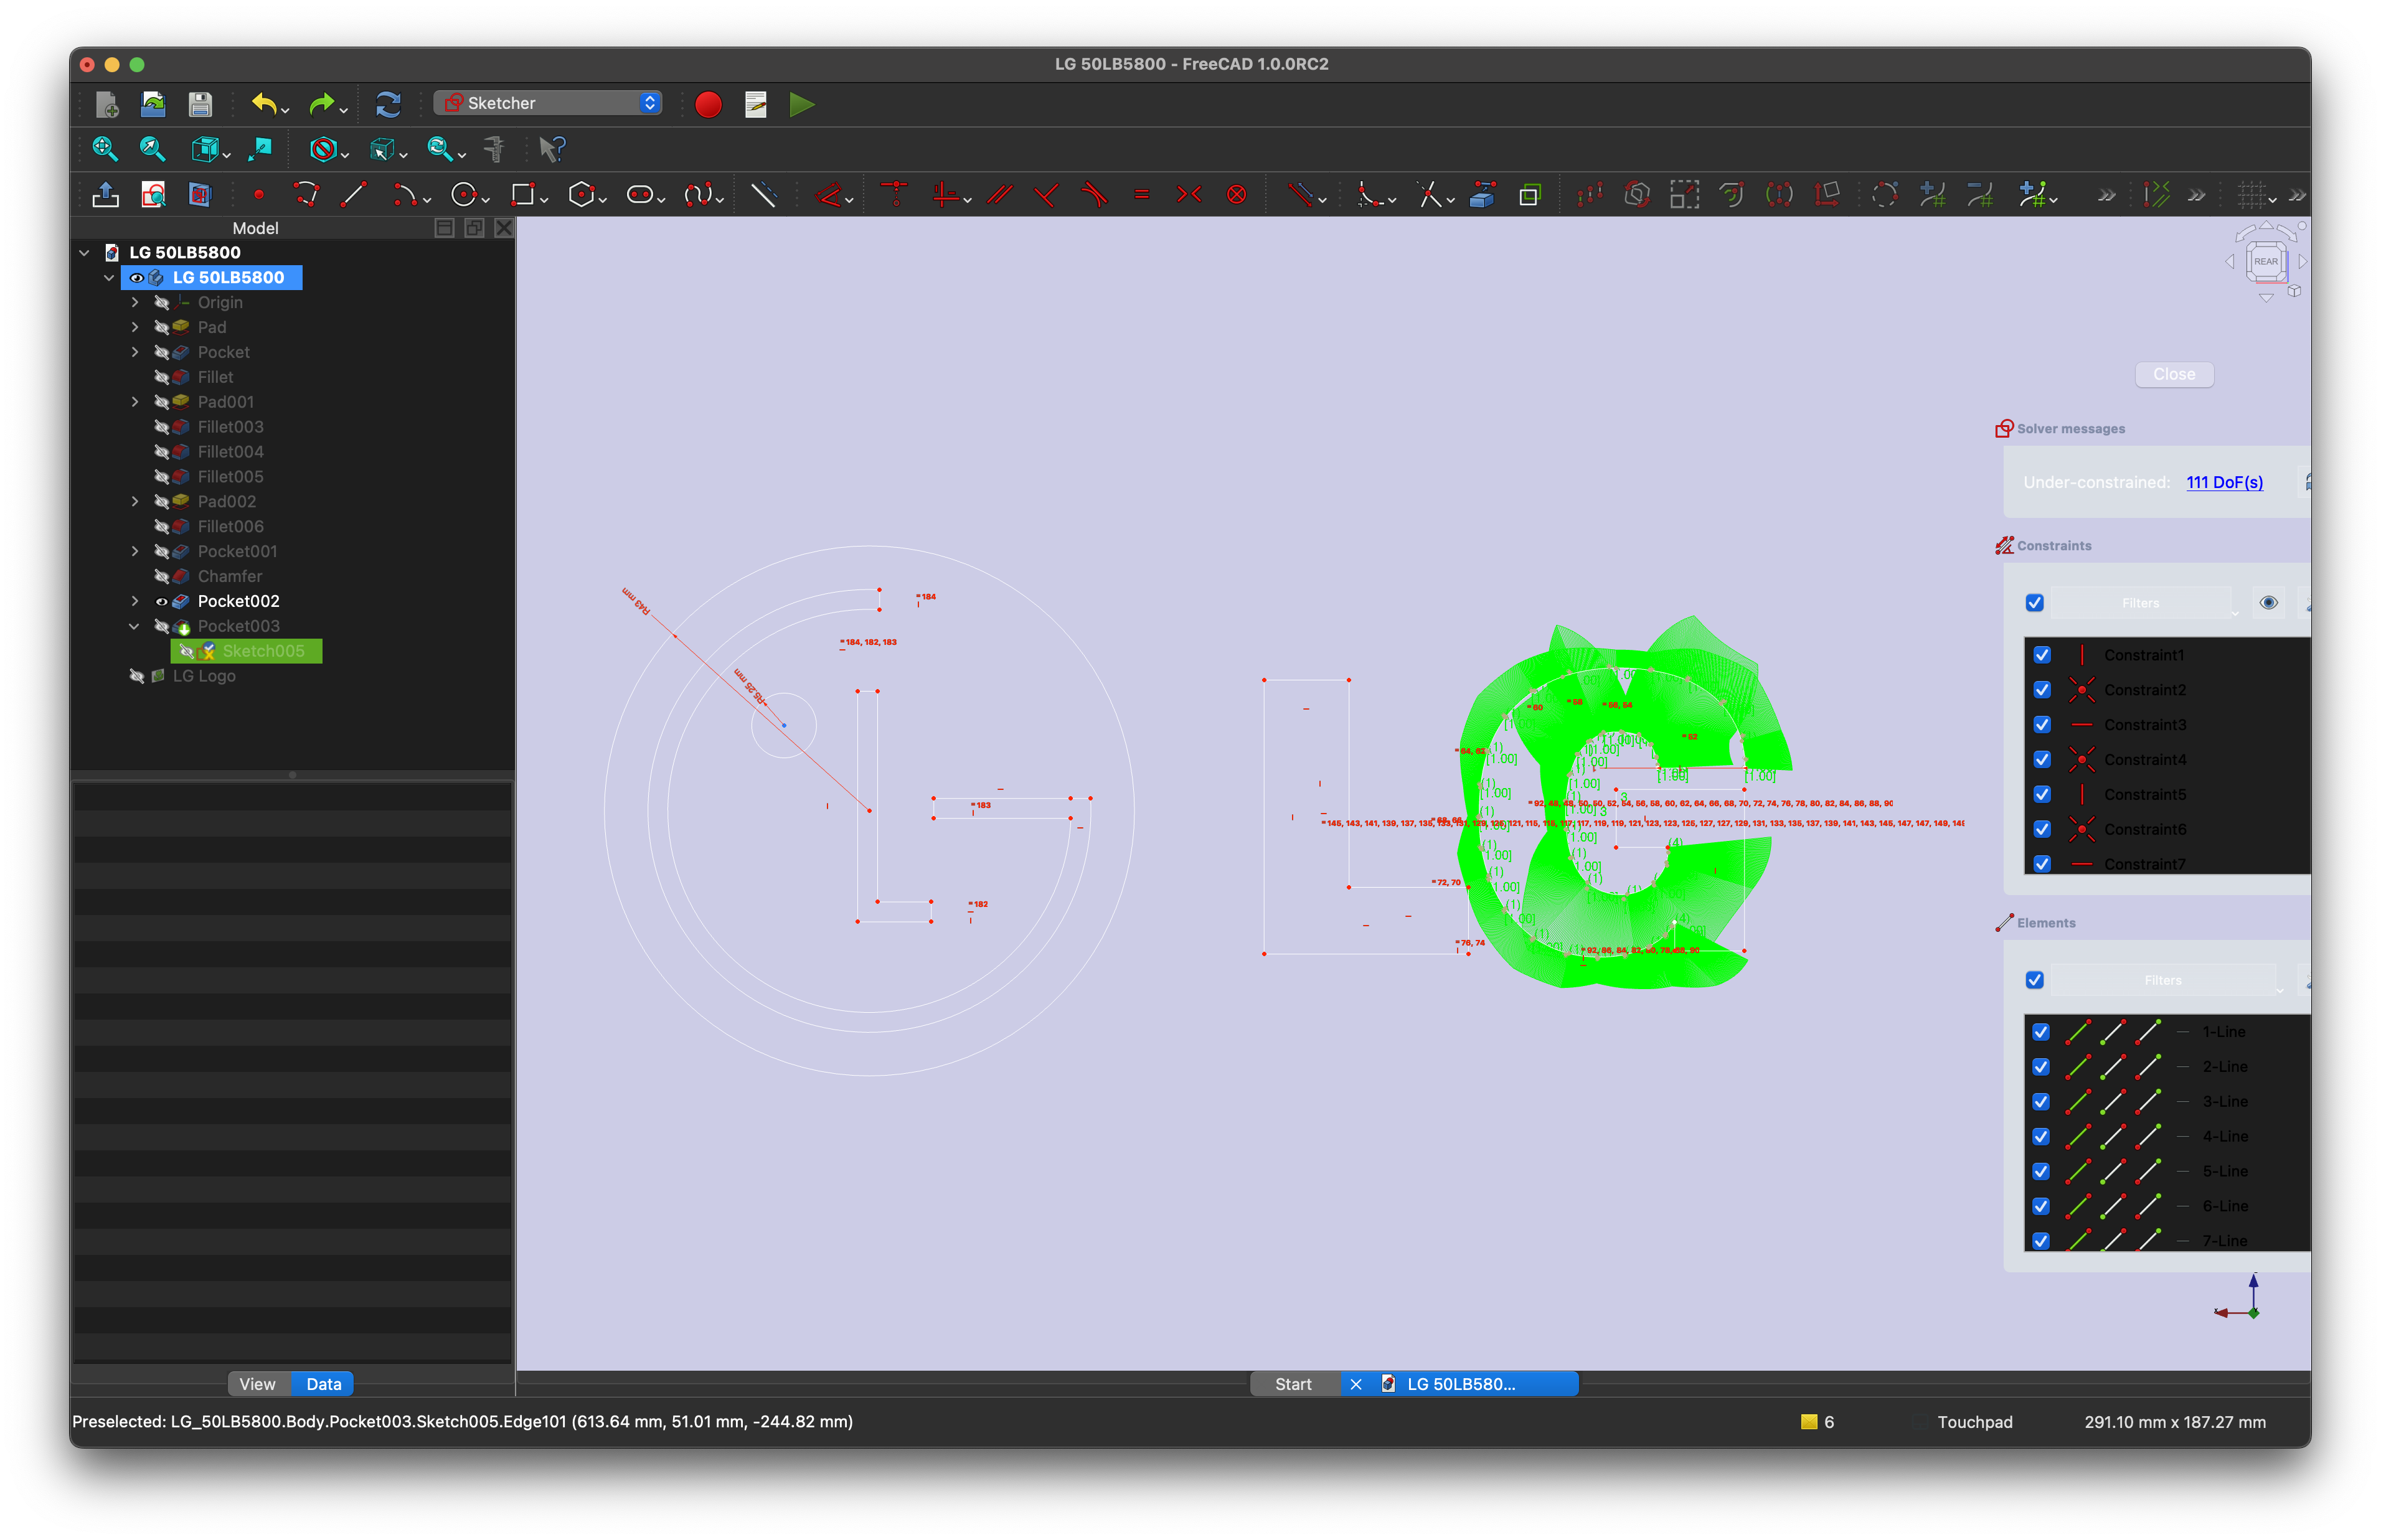
\includegraphics[width=1\linewidth]{a4}
  \caption{Sketching the LG logo on the back of the 3D model.}
  \medskip
  \label{fig:a4}
\end{figure}

Once I was done modelling, I exported my 3D model as an
\href{https://drive.google.com/file/d/1JmbW4QBFge6CosMKm4P-QzFGuzJ4o9Oy/view?usp=sharing}{STL
file} that slicing software can understand. I used
\href{https://ultimaker.com/software/ultimaker-cura}{UltiMaker Cura}
for slicing my model, as it is what Mr. McCallister recommended in
class and is what he showed us the settings for. The settings used
are shown in table \ref{tab:cura-settings}. The model had to be
scaled down for printing, as the 3D printer is small and this print
was only a prototype anyway. The model was scaled in Cura to 15\% of
its original size.

\begin{figure}[H]
  \medskip
  \centering
  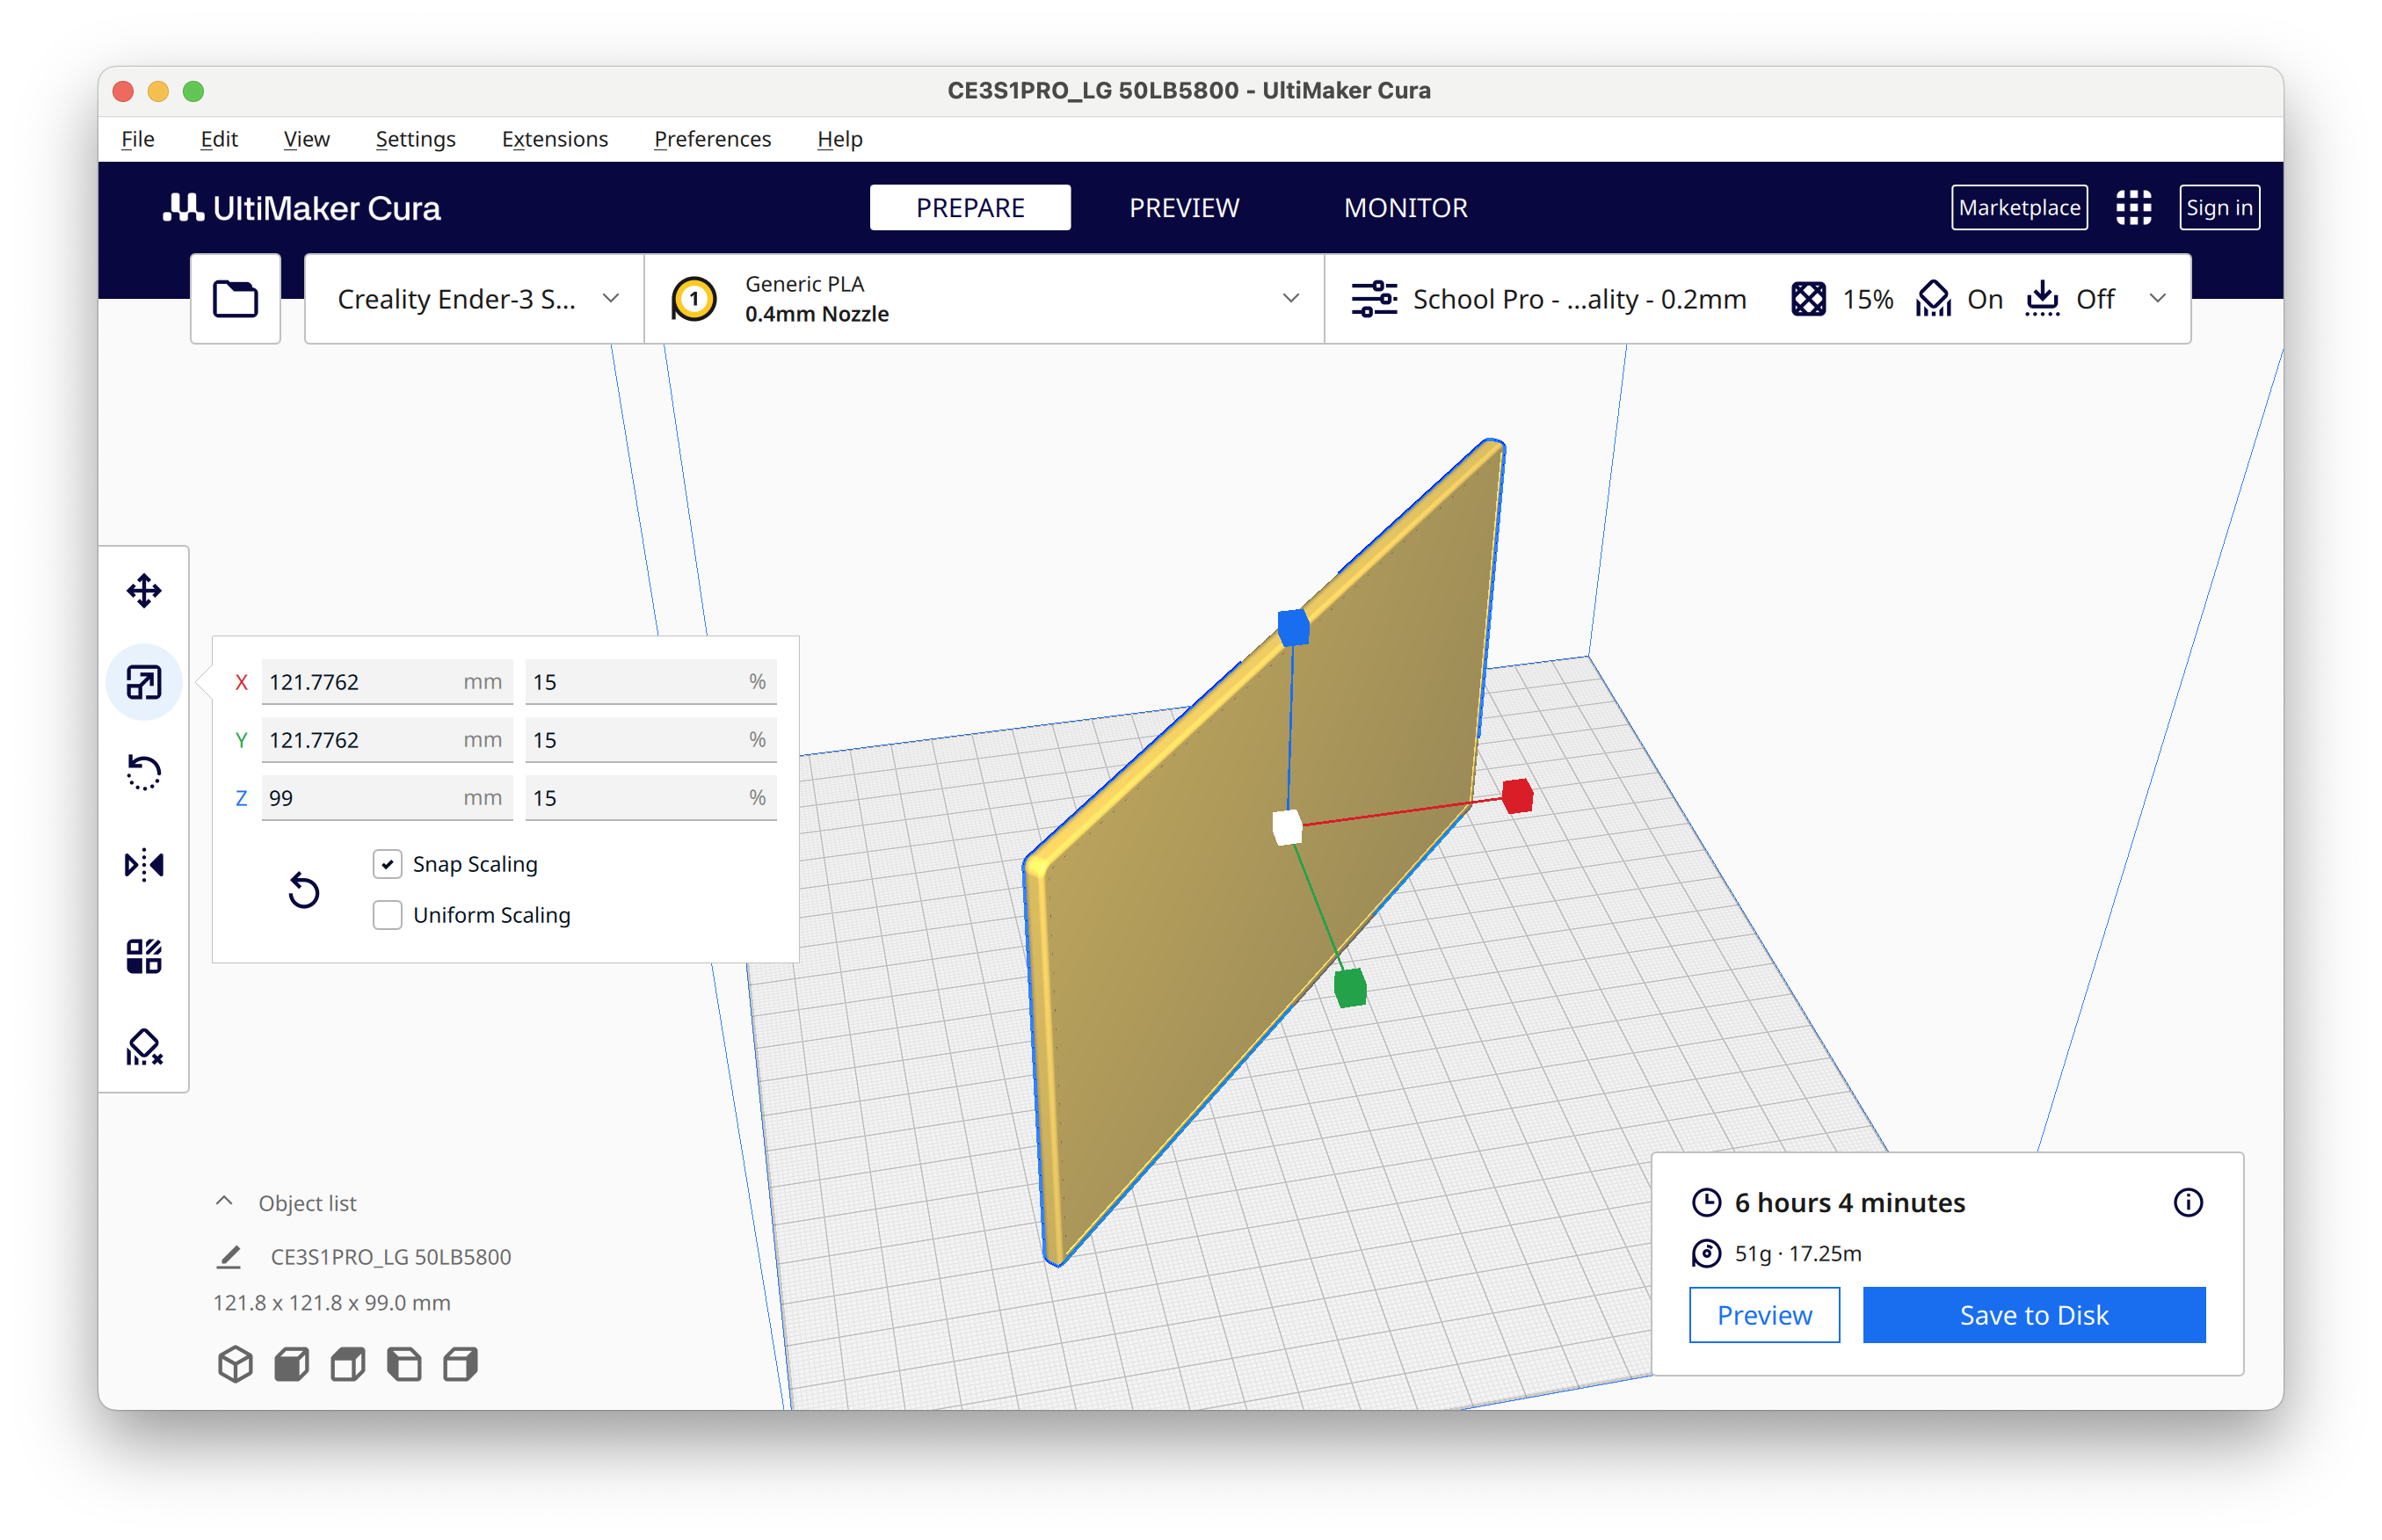
\includegraphics[width=1\linewidth]{a5-cura}
  \caption{Scaling and slicing the 3D model in UltiMaker Cura.}
  \medskip
  \label{fig:a5-cura}
\end{figure}

\begin{table}[H]
  \centering
  \begin{tabular}{ccc}
    Setting & Default Value & New value \\
    \hline
    Infill Density & 20.0\% & 15.0\% \\
    Generate Supports & False & True \\
    Support Structure & Normal & Tree \\
    Printing Temperature & 200.0 \textdegree C & 215.0 \textdegree C \\
  \end{tabular}
  \caption{Settings used for slicing the model in UltiMaker Cura.}
  \label{tab:cura-settings}
\end{table}

Once the model was sliced into G-code, I saved the G-code onto an SD
card and put it in one of the printers. After cleaning the print
plate and applying some glue, I set it off to print. The first two
prints failed, so I tried a different 3D printer and was able to get
it to print well enough.

\todo{Image of the printed 3D model.}

\section{Criterion B}

\subsection{Production Questions and Addressing Strategies}

\begin{itemize}
  \item How does/did LG make the IPS LED displays for its LCD TVs?
    \begin{itemize}
      \item Research LG LCD production process and the role of LG
        Display and LG Chem.
    \end{itemize}

  \item What are the environmental impacts of LG's TV production
    process?
    \begin{itemize}
      \item Research LG's sustainability initiatives and the
        environmental impacts of TV production.
    \end{itemize}

  \item What are the ethical concerns with LG's TV production?

  \item Where are the raw materials for LG's TVs sourced from?
    \begin{itemize}
      \item Research LG's supply chain and raw material sourcing, and
        maybe the role of LG Electronics and LG Chem.
    \end{itemize}
\end{itemize}

\subsection{General Production Process}

This specific model of the 50LB5800 LG Smart TV that I have at home
was assembled in Poland, July 2014, as can be seen on the
informational sticker on the back of the TV in figure
\ref{fig:lg-back-label}. The TV was likely produced in the LG
production plant in Mława, Poland~\autocite{lg-2020}. The LG Display
plant in Mława, however, was relocated to Wrocław in 2016 and is no
longer operated by LG
Display~\autocite{allen-2016}~\autocite{evertiq-ab-2016}, being sold
to LG Chem instead~\autocite{shah-2024}. The TV was likely produced
in the Mława plant before it was relocated. This model of the TV is
also now discontinued and no longer produced~\autocite{unknown-author-no-dateB}.

\begin{figure}[H]
  \medskip
  \centering
  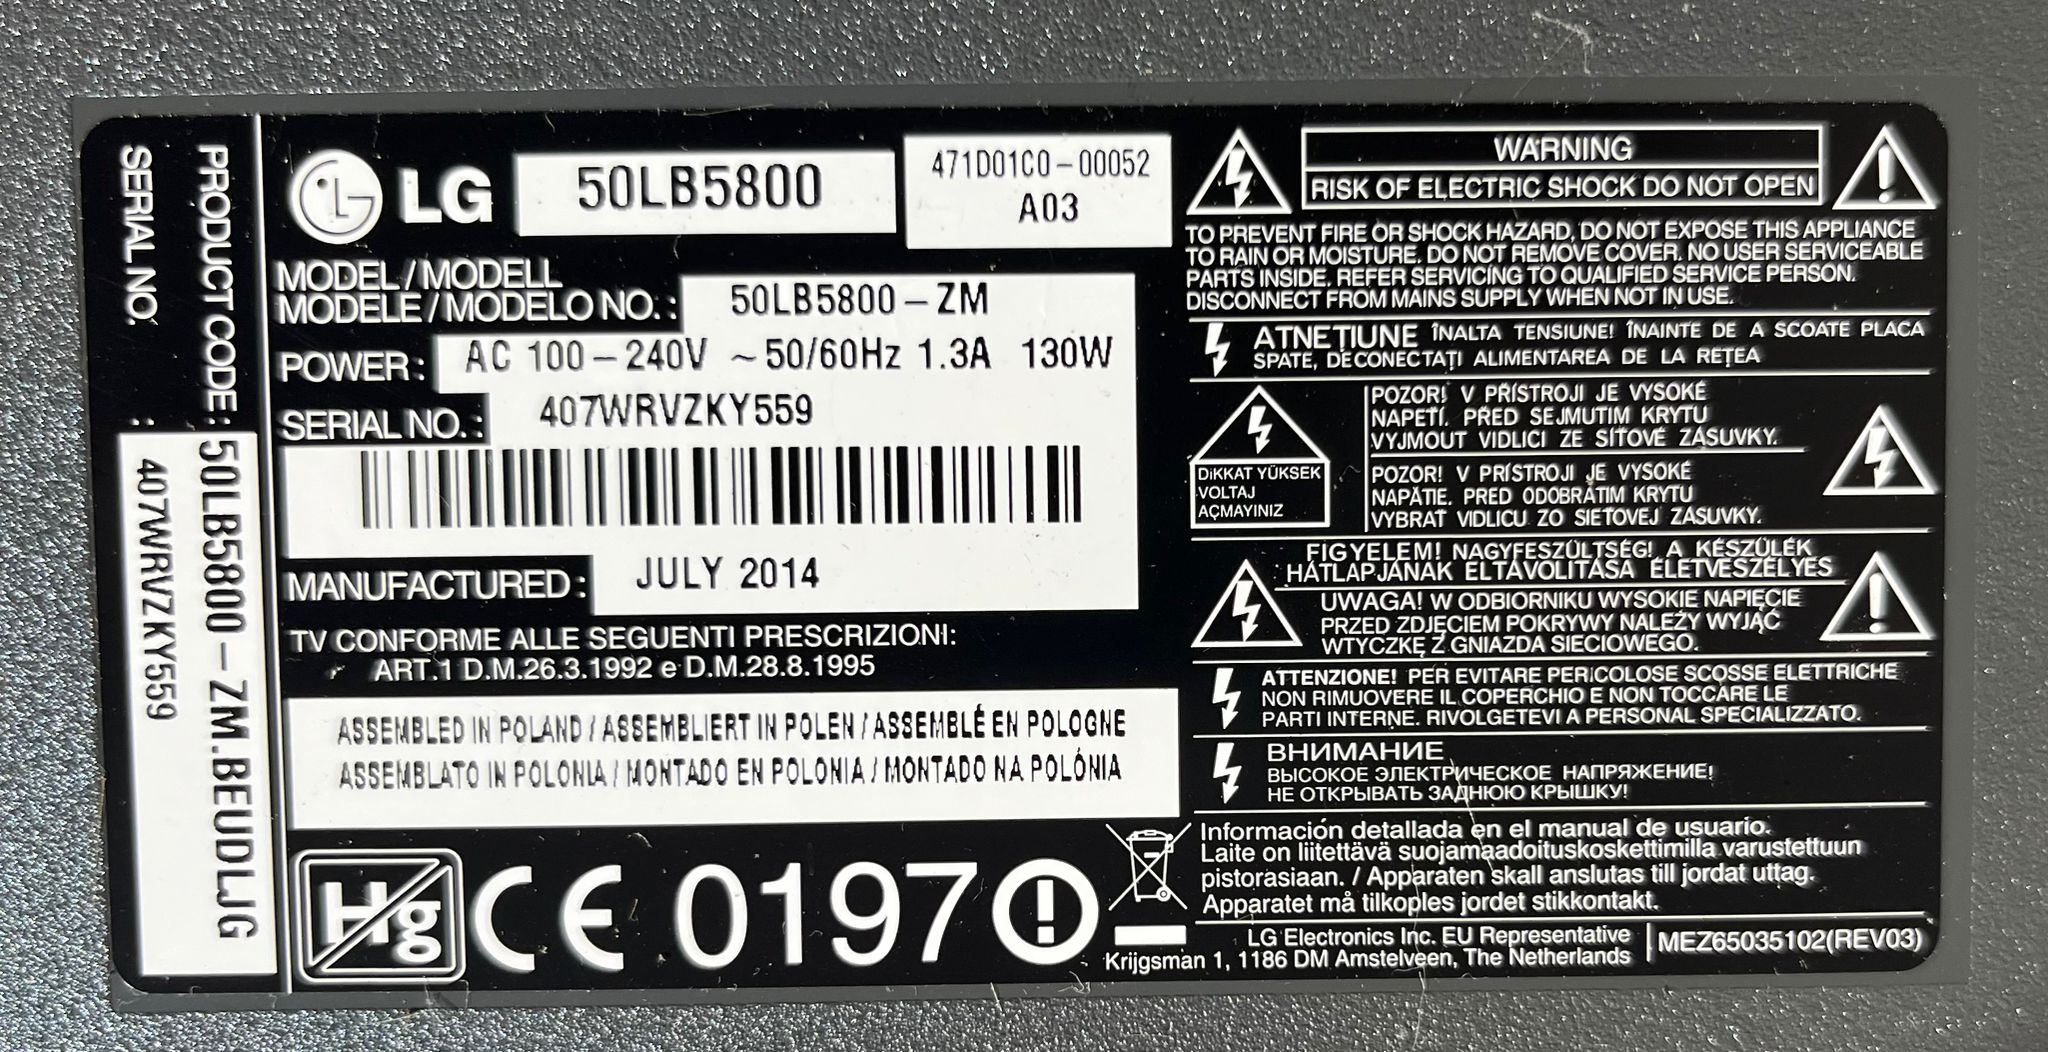
\includegraphics[width=1\linewidth]{lg-back-label}
  \caption{The informational sticker on the back of my LG 50LB5800 Smart TV.}
  \medskip
  \label{fig:lg-back-label}
\end{figure}

\begin{figure}[H]
  \medskip
  \centering
  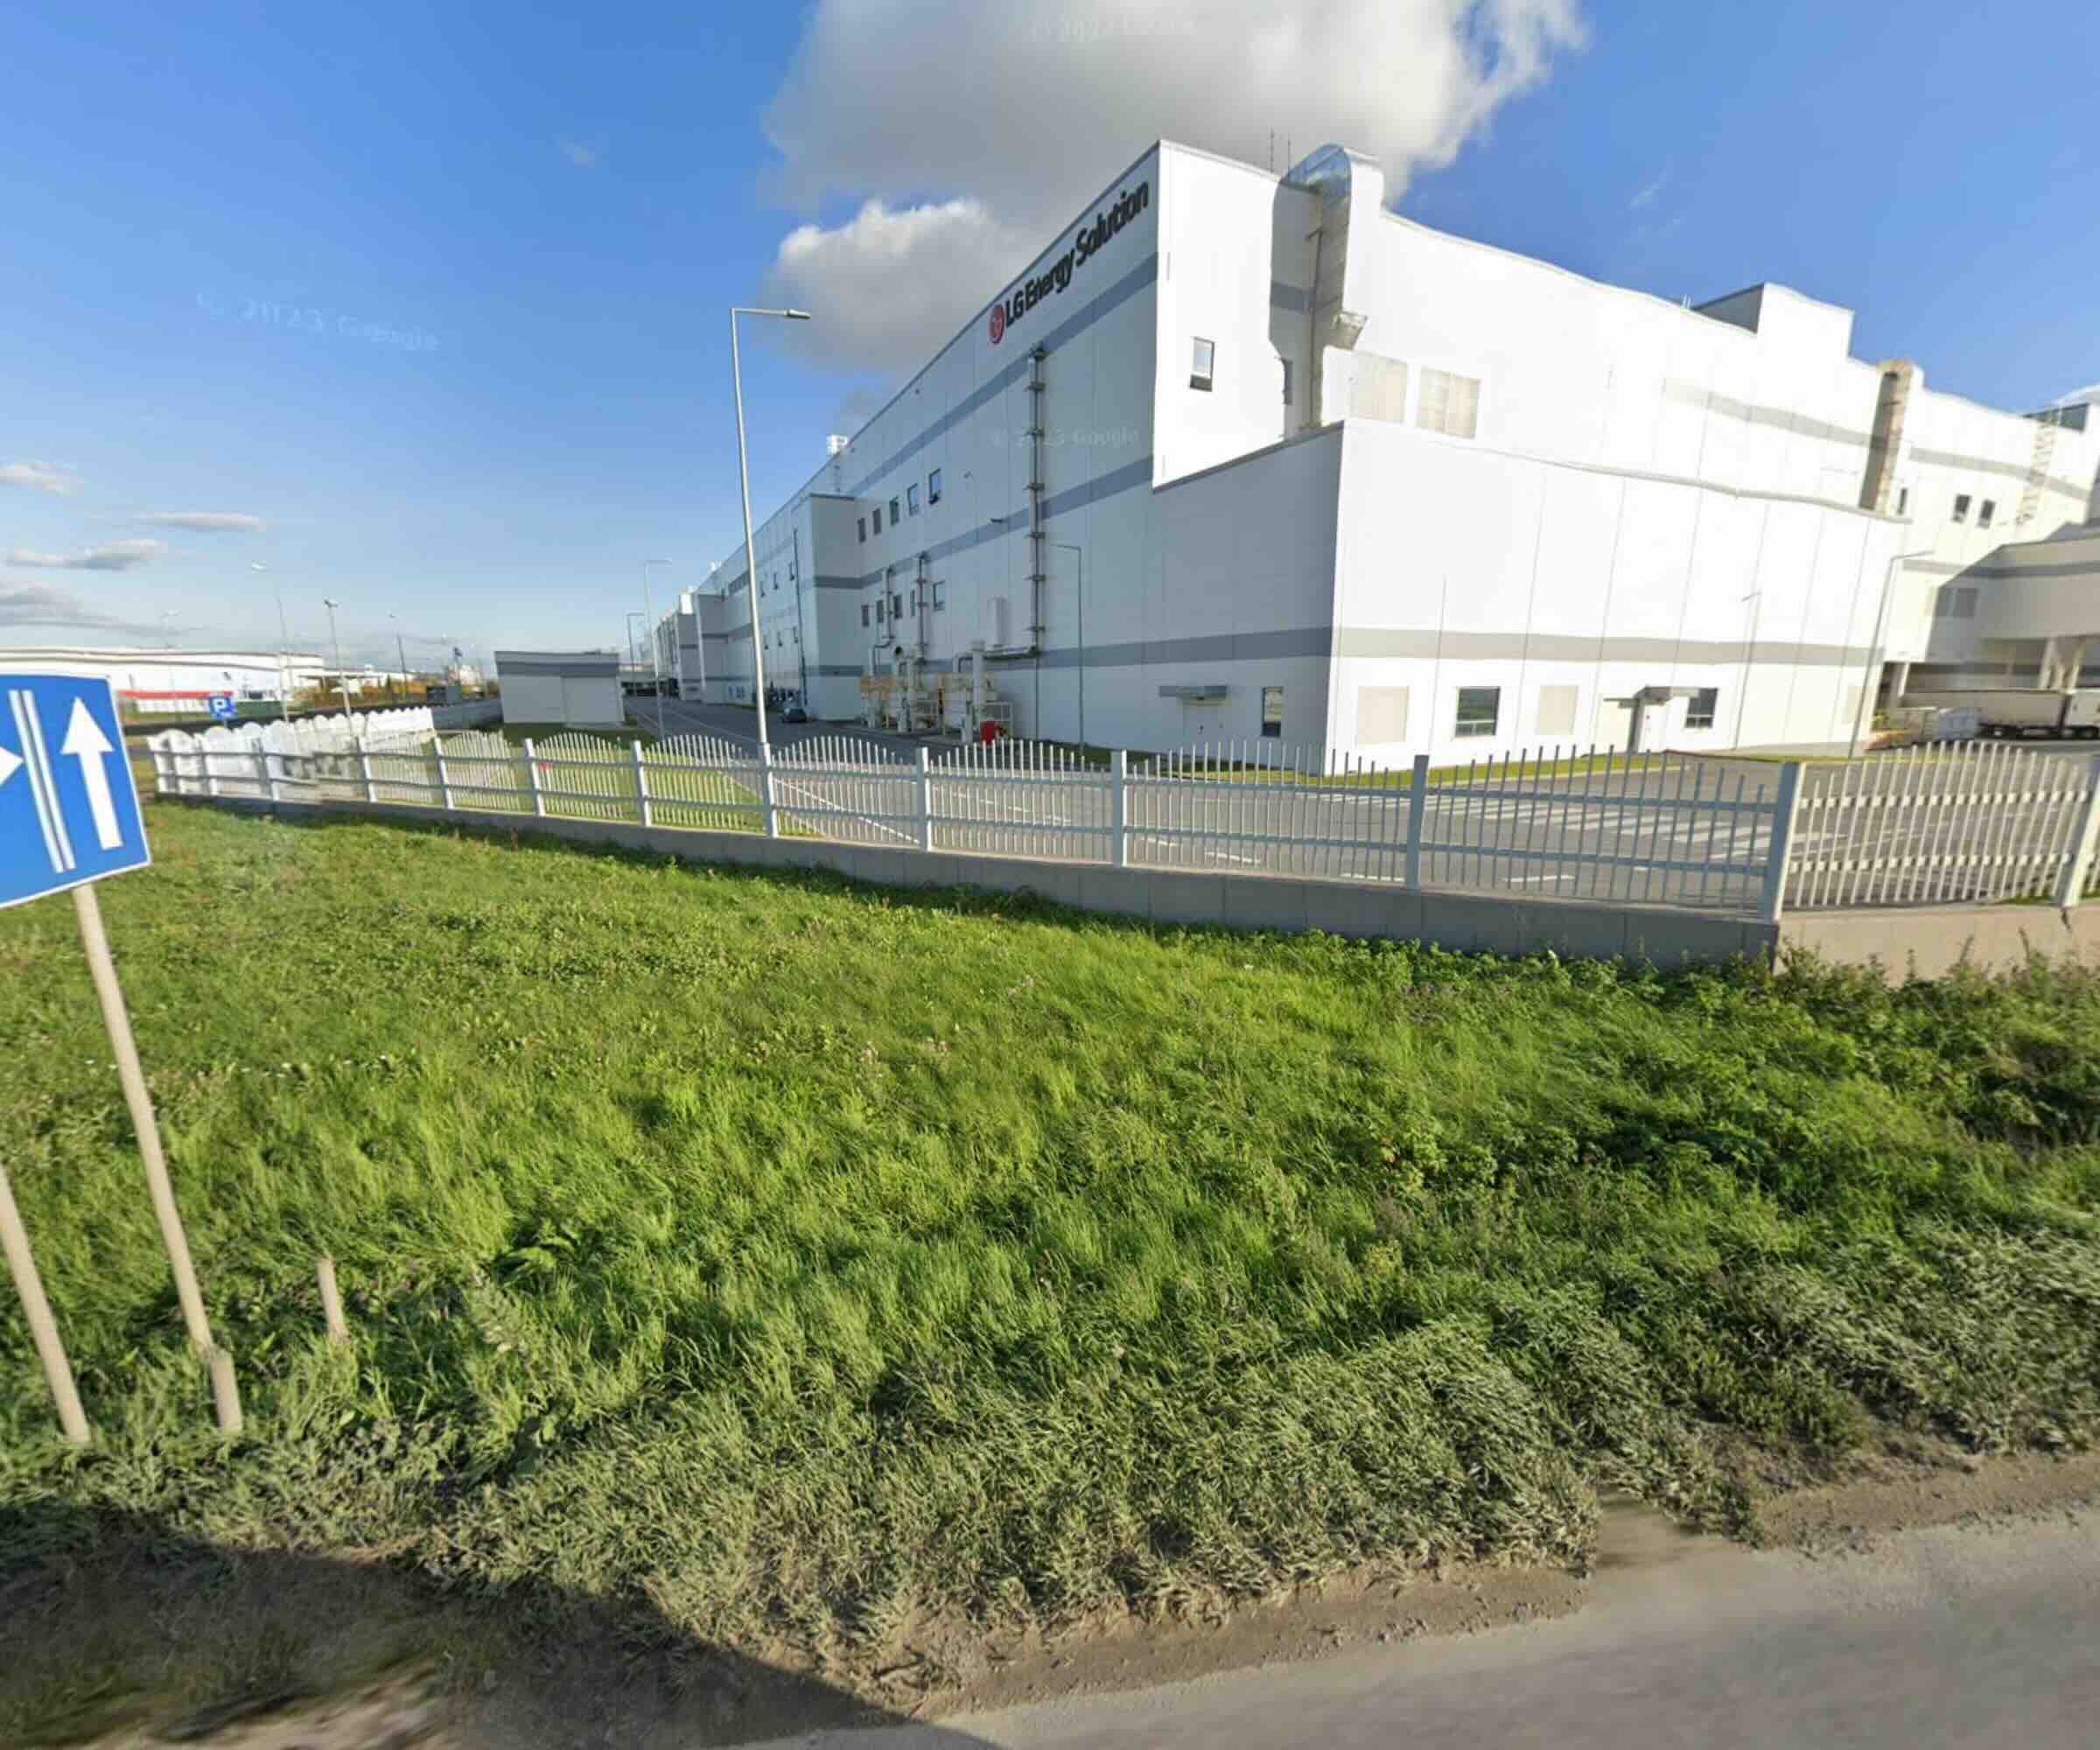
\includegraphics[width=1\linewidth]{lgensol-wroclaw-google-maps}
  \caption{The LG plant in Wrocław, Poland. Image from
  \href{https://maps.app.goo.gl/vMukYzKtPBX12RGo9}{Google Maps}.}
  \medskip
  \label{fig:lgensol-wroclaw-google-maps}
\end{figure}

The production process of the LG 50LB5800 Smart TV is not
specifically documented, but it can be inferred from the general
production process of LG TVs. Jeremy Kaplan, a former editor-in-chief of
Digital Trends, visited the LG Display facility in Gumi, South Korea,
and described the manufacturing process of LG's TVs.

\todo{Explain the general production process of LG TVs.}

\subsection{Ethical Concerns}

As with any electronic device, there are ethical concerns with the
production of LG TVs. The TVs will contain conflict minerals, like
tin, tantalum, tungsten, and gold. These minerals are sourced from
conflict regions, like the Democratic
Republic of the Congo, and are often mined using child labor and
under dangerous conditions~\autocite{hower-2013}. LG has a policy to
avoid using conflict
minerals, but it is difficult to ensure that all minerals are
conflict-free~\autocite{lg-electronics-no-date}. In LG's Policy for
Conflict Materials, LG states the following:

\begin{quote}
  LGE is committed to adopting, widely disseminating and incorporating
  principles in support of these goals in contracts, agreements and/or
  communications with suppliers. LGE expects our suppliers to have in
  place policies and due-diligence measures to facilitate the sourcing
of minerals that are ``DRC conflict free.\textsuperscript{3)}'' In
addition, LGE requires
our suppliers to comply with LGE's Supplier Code of Conduct, based on
the Responsible Business Alliance (RBA) Code of Conduct, which sets
forth LGE's broader standards for suppliers and includes provisions
relating to human rights, ethical conduct, and environmental
protection as well as additional provisions relating to conflict minerals.
\end{quote}

This absolves the main company. It's their way out of taking
responsibility and leaving it up to their suppliers.

\subsection{Raw Materials}

As of 2023, LG has 249 suppliers of conflict minerals in 41
countries. Only two of these are in Poland, both conforming to LG's
audit protocols. One of them is Fenix Metals, a supplier of tin, and
the other is KGHM Polska Mied\'z, a supplier of
gold~\autocite{lg-electronics-2023}. Tin is used for soldering
electronic and metallic components, and gold is used for circuit
board connectors~\autocite{brigham-2023}. An example of where these
minerals are used in the LG 50LB5800 Smart TV is in its mainboard, as
seen in figure \ref{fig:EBT62999602}, which contains gold connectors
and tin soldering.

\begin{figure}[H]
\medskip
\centering
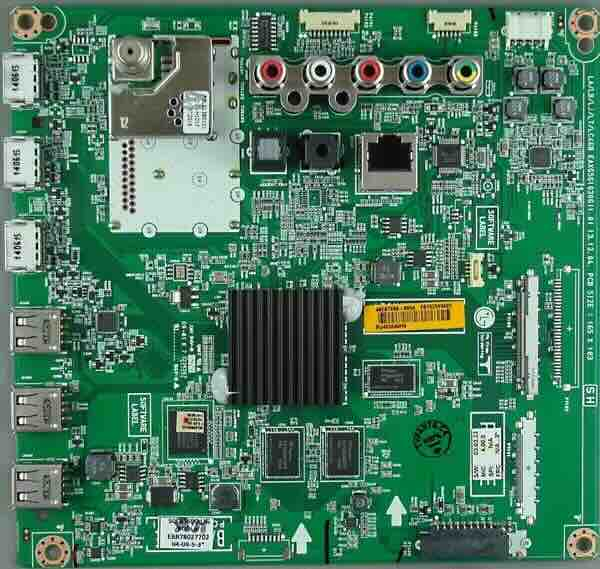
\includegraphics[width=1\linewidth]{EBT62999602}
\caption{The LG 50LB5800 Smart TV mainboard~\autocite{tv-parts-canada-2024}.}
\medskip
\label{fig:EBT62999602}
\end{figure}

The mainboard goes through a surface treatment process called
immersion tin. Immersion tin involves replacing copper with tin on
PCB solder pads, and has several advantages and disadvantages. Some
advantages include increased solderability, versatility, and
environmental friendliness, while some disadvantages include quicker
oxidation and soldering reliability issues~\autocite{jenell-2023}.

Gold is used in several parts of the TV, such as the PCB, connectors
and microchips. Gold is used in gold plating for the PCB for
efficient and reliable electrical connections, in connectors for its
low resistance and good durability, and in microchips for its high
conductivity~\autocite{elmore-2024}.

\printbibliography[heading=bibintoc,title=References]

\end{document}

